\providecommand{\main}{..}
\documentclass[\main/main.tex]{subfiles}


\begin{document}


\subsection{Markov chains} \label{markov_chain}
A Markov chain is a special type of stochastic processes where $X_{t+1}$ depends on $X_{t}$ only, i.e. the probability of the next random outcome depends on the present realisation but it is independent of the past \citep{Grinstead1997}. Clearly, this is one of the simplest form of dependency \citep{Sheskin2010}. More formally, a Markov chain is as \lq\lq an indexed collection of random variables used to model a sequence of dependent events such that the probability of the next event depends only on the present event'' \citep{Sheskin2010}.\\

Markov chain models were introduced in the early 20th century by the Russian mathematician A. A. Markov \citep{Hayes2013}. In the United States, Markov chains  began to gain popularity from the 1950's, when both academia - see for instance, \cite{Feller1950}, \cite{Howard1960}, and \cite{Kemeny1960} - and mathematicians at the RAND Corporation in California started investigating theory and applications of Markov decision processes \citep{Sheskin2010}. Markov chains have now been applied to a variety of problems such as Markovian queueing systems, webpage ranking, inventory control, customer lifetime value etc. \cite{Ching2006} provide an overview and some practical examples of the many fields of application of such models.\\


\subsubsection{Terminology}

As with stochastic processes, the possible values that a Markov chain can assume are called \textit{states}, and the set of these values is called the \textit{state space}. In this setting, we will assume that the states are finite and mutually exclusive $S = \{s_1,s_2,...,s_t, s\}$ and that Markov chain is observed to be in one of them. For instance, if $X_t = s_i$ we say that the Markov chain, or system, is in state $s_i$ at time $t$.\\


The \textit{trajectory}, or \textit{sample path}, will be the set of values that the sequence of random variables assumes over a given time horizon. For instance, when we observe $X_0 = s_0, X_1 = s_1, X_2 = s_2, ...$, we say that the Markov chain has trajectory $s_0, s_1, s_2,...$. 

The sequence of random variables is typically observed at equally spaced points in time, called 
\textit{epochs}. An epoch is denoted by $t = 0, 1, 2, ...$ . Epoch $t$ designates the end of time period $t$ and the beginning of period $t + 1$. The time interval between two successive epochs is called \textit{period or step}. \citep{Sheskin2010}.\\


\begin{figure}[H]
\centering
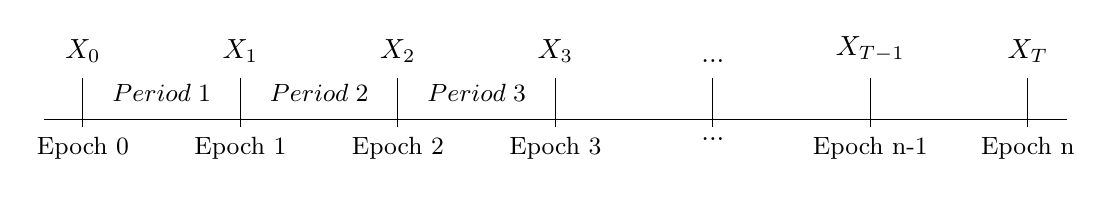
\begin{tikzpicture}
% draw horizontal line   
\draw (-0.5,0) -- (12.5,0);
% draw vertical lines
\foreach \x in {0,2,4,6,8,10,12}
\draw (\x cm,15pt) -- (\x cm,-3pt);
% draw nodes
\draw (0,0) node[below=3pt] {\small Epoch  0} node[above=3pt] {$   $};
\draw (0,0) node[above=17pt] {$X_0$} node[above=3pt] {};
\draw (2,0) node[above=17pt] {$X_1$} node[above=3pt] {};
\draw (4,0) node[above=17pt] {$X_2$} node[above=3pt] {};
\draw (6,0) node[above=17pt] {$X_3$} node[above=3pt] {};
\draw (8,0) node[above=17pt] {$...$} node[above=3pt] {};
\draw (10,0) node[above=17pt] {$X_{T-1}$} node[above=3pt] {};
\draw (12,0) node[above=17pt] {$X_{T}$} node[above=3pt] {};
\draw (1,0) node[below=3pt] {} node[above=3pt] {\small $Period \; 1$};
\draw (2,0) node[below=3pt] { \small Epoch 1} node[above=3pt] {};
\draw (3,0) node[below=3pt] {$  $} node[above=3pt] {\small $Period \; 2$};
\draw (4,0) node[below=3pt] {\small Epoch 2} node[above=3pt] {};
\draw (5,0) node[below=3pt] {} node[above=3pt] {\small $Period \; 3$};
\draw (6,0) node[below=3pt] {\small Epoch 3} node[above=3pt] {$  $};
\draw (8,0) node[below=3pt] {$...$} node[above=3pt] {$  $};
\draw (10,0) node[below=3pt] {\small Epoch n-1} node[above=3pt] {$  $};
\draw (12,0) node[below=3pt] {\small Epoch n} node[above=3pt] {$  $};
\end{tikzpicture}
\caption{Epochs and time periods of a Markov chain}
\label{fig:markov_chain}
\end{figure}






\subsubsection{The Markov property}

The essential feature of Markov chains is that the probability of the next realisation only depends on the current state of the process. In mathematical jargon, this is called \lq\lq the Markov property". Indeed, a Markov chain is defined as \lq\lq an indexed sequence of random variables, $\{X_0, X_1, X_2, ...\}$ that satisfies the Markov property'' \citep{Sheskin2010}. This means that, given the present state of the random process, the conditional probability of the next state depends only on the present state and it is independent of previous states.\\
In other words, \lq\lq only the most recent point in the trajectory affects what happens next'' \citep{Holmes2015}.
The \lq\lq Markov property" in formula can be expressed as:

\begin{equation}
\begin{split}
     & \mathds{P} \big(X_{t+1} = s |X_t = s_t, X_{t-1} = s_{t-1}, . . . , X_0 = s_0\big) = 
     \mathds{P} \big(X_{t+1} = s |X_t = s_t\big)\\
    & \text{for all} \; t = 1, 2, 3, ... \; \text{and for all states} \; s_0, s_1, . . . , s_t, s.\\
\end{split}
\end{equation}


\subsubsection{How to describe Markov chains}

Markov chains can be describes through \textit{transition diagrams} or \textit{transition matrices}.

A transition diagram visually represents a Markov chain using nodes for states and directed links for the probability of moving from one state to another \citep{Gagniuc2017}. 

A transition matrix collects the transition probabilities $p_{ij}$ and it is usually indicated by the capital letter $\mathbf{P}$. 
Much of the literature on Markov chains considers row-stochasticity (i.e. the probabilities on each row of the matrix sum to 1). However, there are authors that prefer setting matrices as column-stochastic, see for example \cite{Caswell2006}. In this context, we will adopt Caswell's formulation and consider a transition matrix $\mathbf{P}$ of the form:


\begin{center}
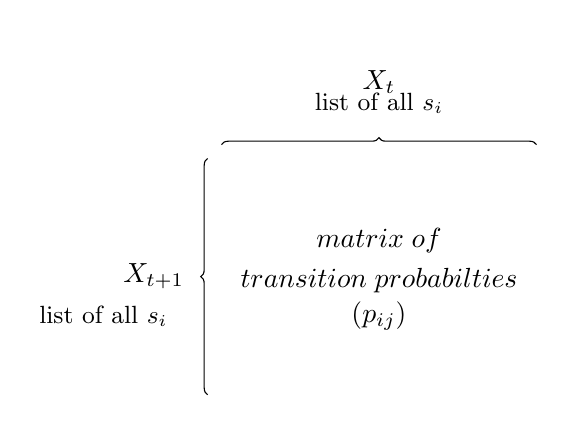
\begin{tikzpicture}
\node[circle,label={$matrix\; of$}] at (2,1.5) {};
\node[circle,label={$transition \; probabilties$}] at (2,1) {};
\node[circle] at (2,1) {$(p_{ij})$};
\node[circle] at (2,3.7) {\small list of all $s_i$};
\node[circle] at (-1.5,1) {\small list of all $s_i$};
\draw[decoration={brace,raise=5pt},decorate]
  (0,0) -- node[left=10pt] {$X_{t+1}$} (0,3);
\draw[decoration={brace,raise=5pt},decorate]
  (0,3) -- node[above=20pt] {$X_t$} (4,3);
\end{tikzpicture}
\end{center}

\noindent Without loss of generality, suppose that the state space has dimension $N$, i.e. $S = \{1, 2, . . . ,N\}$. The $\mathbf{P}$ matrix will be a square $N \times N $ matrix where each column represents the possible states in the current epoch $t$ and each row the possible states in the next epoch $t+1$. Since the transition probabilities are conditioned on the present epoch, the entries of each column sum to one.\\

\noindent Here below you find a minimal example taken from \cite{Sheskin2010} of a transition matrix and a transition diagram that can be used to represent a simple Markov Chain:

\begin{equation}
   \mathbf{P} =
   \begin{pmatrix}
   p_{11} & p_{21} \\ 
p_{12}& p_{22} \\ 
   \end{pmatrix}
\end{equation}

and the corresponding transition diagram:\\
\begin{center} 
\begin{tikzpicture}
\node[state] (q2) {$State \; 1$};
\node[state, right of=q2] (q3) {$State \; 2$};
\draw (q2) edge[loop left] node {$p_{11}$} (q2);
\draw (q3) edge[loop right] node {$p_{22}$} (q2);
\draw (q2) edge[bend left] node {$p_{12}$} (q3);
\draw (q3) edge[bend left] node {$p_{21}$} (q2);
\end{tikzpicture}
\end{center}






\subsubsection{The transition probabilities}
In order to compute the transition probabilities of a Markov chain, we can imagine the process starting in state $i$ and then moving in steps through the other states. \\
Let $\mathds{P}(X_t = i)$ be the probability that the Markov chain is in state $i$ at epoch $t$ and let $\mathds{P}(X_{t+1} = j)$ be the probability that the chain will be in state $j$ in the next epoch $t+1$. Then, $\mathds{P}(X_{t+1}
= j|X_{t} = i)$ will be conditional probability of the Markov chain. i.e. the probability that the process will be in state $j$ at epoch $t + 1$, given that it is in state $i$ at epoch $t$. 
This conditional probability is called the \textit{transition probability} and it is alternatively denoted by $p_{ij}$ \citep{Sheskin2010}. Note that it refers to the the probability of moving from state $i$ to state $j$ in \textit{one step}  :

\begin{equation}
    p_{ij} = \mathds{P}(X_{t+1} = j |X_t = i) \; \; \text{for}\; \; i,j \in S, \; \; t=0,1,2,...
\end{equation}
Clearly, since the Markov chain must be in some state at time $t+1$ we have \citep{Howard1960}:
\begin{equation}
 \sum_{j=1}^N     p_{ij} = 1
\end{equation}
where $S=\{1,2,...,N\} $. Moreover, since the $p_{ij}$ are probabilities:
\begin{equation}
 0 \leq p_{ij} \leq 1
\end{equation}\\

An additional assumption is that transition probabilities are \textit{stationary} over time (or \textit{time homogeneous)} meaning that they do not change over time \citep{Sheskin2010}. If this is the case, it follows that:
\begin{equation}
    p_{ij} = \mathds{P}(X_{t+1} = j |X_t = i)  = \; \; \mathds{P}(X_{0} = j |X_1 = i)
\end{equation}


\noindent Finally, the Markov chain evolves over time and \lq\lq visits'' a sequence of states, thereby originating a \lq\lq trajectory''. The probability of such trajectory, e.g. $X_0 = a, X_1 = b, X_2 = c$ is a joint probability that can be computed taking into account the Markov property:

\begin{equation}
\begin{split}
   &\mathds{P}(X_0 = a, X_1 = b, X_2 = c) =\\
   =\;  &\mathds{P}(X_0 = a) \mathds{P}(X_1 = b |X_0 = a ) \mathds{P}(X_2 = c |X_1 = b ) = \\
   =\; &p_a \; p_{ab}\; p_{bc}
\end{split}
\end{equation}
where $p_a$ represent the probability that the initial state is equal to $a$. Since the initial state is usually known $p_a = 1$, the above formula simplifies:
\begin{equation}
\begin{split}
   &\mathds{P}(X_0 = a, X_1 = b, X_2 = c) =\\
   =\; &p_{ab}\; p_{bc}
\end{split}
\end{equation}







\subsubsection{T-step transition probabilities of the transition matrix}

Let $\{X_0, X_1, X_2, \cdots \}$ be a Markov chain with state space $S = \{1, 2, . . . ,N\}$. There are different but equivalent methods to retrieve the transition probabilities over different steps. The following is based on \cite{Holmes2015} and \cite{Sheskin2010}. \\

\noindent\textit{One-step transition probabilities}\\
\noindent The one-step transition probabilities are the entries $p_{ij}$ of the matrix $\mathbf{P}$. Indeed, by definition:

\begin{equation}
    p_{ij} = \mathds{P} ( X_{t+1} = j | X_t = i)
\end{equation}
where the entries of $\mathbf{P}$ represent the probability of making a transition from state $i$ to state $j$ in a one single step.\\

\noindent \textit{Two-step transition probabilities}\\
\noindent The two-step transition probabilities $p_{ij}^2$ represent the probability of making a transition from state $i$ to state $j$ in two steps. To calculate a two-step transition probability one can reason in the following way \citep{Sheskin2010}: $p_{ij}^2$ is the conditional probability of going from state $j$ to state $i$ in two steps, i.e. passing through an intermediate state $k$, where $k$ can be any of the states of the Markov chain. Thus, the $p_{ij}^2$ can be computed as the product of a first and the second transition probability: the first transition is from state $i$ to state $k$ and the second is from state $k$ to $j$. Since the value of $k$ is unknown, we have sum over all the possible state of $k$. This idea relies on the law of total probability \citep{Zwillinger2000}.

To give a simple example, suppose the state space of the Markov chain is $S = \{ 1,2,3\}$:

\begin{equation}
    p_{ij}^2 = p_{i1}p_{1j} + p_{i2}p_{2j} + p_{i3}p_{3j} = \sum_k p_{ik}p_{kj}
\end{equation}

\noindent The matrix $\mathbf{P}^{(2)}$ collects all the two-step transition probabilities. By the rules of matrix multiplication, the matrix $\mathbf{P}^{(2)}$ can be obtained by multiplying the one-step transition matrix by itself:
\begin{equation}
    \mathbf{P}^{(2)} = \mathbf{P} \mathbf{P} = \mathbf{P}^2 
\end{equation}\\

\begin{equation}
\begin{split}
  \mathbf{P}^2 = \mathbf{P} \mathbf{P} &= 
\begin{bmatrix}
p_{11} & p_{21} & p_{31} \\
p_{12} & p_{22} & p_{32}  \\
p_{13} & p_{23} & p_{33}  \\
\end{bmatrix}
\begin{bmatrix}
p_{11} & p_{21} & p_{31} \\
p_{12} & p_{22} & p_{32}  \\
p_{13} & p_{23} & p_{33}  \\
\end{bmatrix}=\\
&= 
\begin{bmatrix}
p_{11}p_{11} + p_{21}p_{12} + p_{31}p_{13} & \cdots \\
\vdots\\
\end{bmatrix} =
\begin{bmatrix}
p_{11}p_{11} + p_{12}p_{21} + p_{13}p_{31} & \cdots \\
\vdots\\
\end{bmatrix} =\\
&= 
\begin{bmatrix}
\sum_{k=1}^3 p_{1k}p_{k1} & \cdots\\
\vdots\\
\end{bmatrix} = 
\begin{bmatrix}
\sum_{k=1}^N p_{ik}p_{kj} & \cdots\\
\vdots\\
\end{bmatrix} = 
\mathbf{P}^{(2)} 
\end{split}
\end{equation}

\noindent \textit{T-step transition probabilities}\\
The idea for the two-step transition matrix can be shown (see Appendix) to extend to the more general case. Indeed, the t-step transition matrix is equal to the  $t^{th}$ power the one-step transition matrix:

\begin{equation}
    \mathbf{P}^{(t)} = \mathbf{P}^t
\end{equation}

\noindent Let $B_1, B_2, ..., B_n$ be a collection of mutually exclusive and exhaustive events (i.e. they are a set of pairwise disjoint events $B_i \cap B_j = \varnothing \; \; \forall \; \; i, j$ whose union is the entire sample space $\Omega$) with $\mathds{P}(B_i) \neq 0 \; i=1,2,...,n$, then for every event  $A$:
\begin{equation}
     \mathds{P}(A) = \sum_{i=1}^{n} \mathds{P} (A \cap B_i) = \sum_{i=1}^{n} \mathds{P}(A | B_i) \mathds{P}(B_i) \; \; \text{for every event A}
\end{equation}
where the last equality follows from the definition of conditional probability:

\begin{equation}
    \mathds{P}(A | B_i) = \frac{\mathds{P}(A \cap B_i)}{\mathds{P}(B_i)}
\end{equation}

\noindent To ease notation, I will use interchangeably $X(t+i) = X_{t+i}$ and $\mathds{P} ( X_{t+2} = j | X_t = i) =  \mathds{P}_i ( X_{t+2} = j)$.
Applying the above results to the two-step transition probability, we obtain \citep{Holmes2015CourseProcesses}:


\begin{equation}
\begin{split}
&\mathds{P} ( X_{t+2}= j | X_t = i) = \mathds{P}_i ( X_{t+2}) = \; \; \; \; \; \;  \text{(change in notation)}\\
&= \sum_{k= 1}^{N}  \mathds{P}_i  ( X_{t+2} = j \cap X_{t+1} = k) = \; \; \; \; \; \;  \text{(total law of probability)}\\
&= \sum_{k= 1}^{N} \mathds{P}_i  ( X_{t+2} = j | X_{t+1} = k)\; \mathds{P}_i  (X_{t+1} = k) = \; \; \; \; \; \;  \text{(def. of conditional probability)}\\
&= \sum_{k= 1}^{N} \mathds{P}  ( X_{t+2} = j | X_{t+1} = k, X_{t} = i)\; \mathds{P}  (X_{t+1} = k | X_{t} = i) = \; \; \; \; \; \;  \text{(change in notation)}\\
&= \sum_{k= 1}^{N} \mathds{P}  ( X_{t+2} = j | X_{t+1} = k)\; \mathds{P}  (X_{t+1} = k | X_{t} = i) = \; \; \; \; \; \;  \text{(Markov property)}\\
&= \sum_{k= 1}^{N} p_{kj}p_{ik} \; \; \; \; \; \;  \text{(by def.)}\\
&= \sum_{k= 1}^{N} p_{ik}p_{kj} \; \; \; \; \; \;  \text{(rearranging)}\\
&= (P^2)_{ij} \; \; \; \; \; \;  \text{(see squared matrix)}\\
\end{split}
\end{equation}

The two-step transition probabilities are therefore given by the matrix $\mathbf{P^2}$.\\


\noindent \textit{Three-step transition probabilities}\\

The three-step transition probability is found similarly, conditioning on the state of the Markov chain at time 2:

\begin{equation}
\begin{split}
&\mathds{P}( X_{t+3}= j | X_t = i) =\\
&= \sum_{k= 1}^{N} \mathds{P}_i( X_{t+3} = j \cap X_{t+2} = k) =\\
&= \sum_{k= 1}^{N} \mathds{P}_i( X_{t+3} = j | X_{t+2} = k)\; \mathds{P}_i(X_{t+2} = k)=\\
&= \sum_{k= 1}^{N} \mathds{P}( X_{t+3} = j | X_{t+2} = k,X_{t} = i)\; \mathds{P}(X_{t+2} = k | X_{t} = i)=\\
&= \sum_{k= 1}^{N} \mathds{P}( X_{t+3} = j | X_{t+2} = k)\; \mathds{P}(X_{t+2} = k | X_{t} = i)=\\
&=\sum_{k= 1}^{N} p_{kj} \; (P^2)_{ik} =\\
&= (P^3)_{ij}
\end{split}
\end{equation}


\noindent \textit{Theorem}\\
Let $\{X(0), X(1), X(2), . . .\}$ be a Markov chain with $N \times N$ transition matrix $\mathbf{P}$, the t-step transition probabilities are given by the matrix $P^t$ for any $t$:
\begin{equation}
\mathds{P}(X(t) = j |X(0) = i) = (P^t)_{ij}
\end{equation}

\noindent It also follows that:
\begin{equation}
\mathds{P}(X(n+t) = j |X(n) = i) = (P^t)_{ij} \;\; \text{for any n} 
\end{equation}

\end{document}



